\documentclass[xcolor=dvipsnames]{beamer}
\usetheme{Boadilla}

\definecolor{HKARedPrim}{RGB}{215, 34, 5}
\definecolor{HFUGreenSec}{RGB}{0, 132, 77}
\definecolor{HFUGrey}{RGB}{218, 220, 220}
\definecolor{HFUAnthr}{RGB}{112, 113, 115}
\usecolortheme[named=HKARedPrim]{structure}
\setbeamertemplate{section in toc}[circle]
\setbeamertemplate{subsection in toc}[square]

\setbeamertemplate{frametitle}{\vspace{0.9em}\textbf{\insertframetitle}}

\usepackage[T1]{fontenc}
\usepackage[english]{babel}
\usepackage{graphicx}
\usepackage{eso-pic}
\usepackage{caption}

\usepackage{listings}
\lstdefinestyle{customc}{
	belowcaptionskip=1\baselineskip,
	breaklines=true,
	numbers=left,
	columns=flexible,
	xleftmargin=2em,
	xrightmargin=1em,
	firstnumber=1,
	numberfirstline,
	numberstyle=\tiny\sffamily,
	numbersep=6pt,
	basicstyle=\footnotesize\ttfamily,
	keywordstyle=\bfseries\color{green!40!black},
	commentstyle=\itshape\color{purple!40!black},
	identifierstyle=\color{blue},
	backgroundcolor=\color{gray!10!white},
}
\lstset{style=customc}
\lstset{captionpos=b}

\title[PA2]{\textbf{Seminararbeit}}
\subtitle{Dynamische Programmanalysen für nebenläufige Programme - Data Race Prediction mit TSan}
\author[Frank Ling]{
\includegraphics[trim={1230px 0 0 0}, clip, scale=0.1]{pics/HKA_Logo_Logoleiste_RGB.png}\\Frank Ling}
\date{13. Juni 2023}
\setbeamertemplate{itemize item}{$\circ$}

\begin{document}
	
	\frame{\titlepage}
	
	\newcommand\AtPagemyUpperLeft[1]{\AtPageLowerLeft{%
			\put(\LenToUnit{0.6\paperwidth},\LenToUnit{0.86\paperheight}){#1}}}
	\AddToShipoutPictureFG{
		\AtPagemyUpperLeft{{
\includegraphics[scale=0.06]{pics/HKA_Logo_Logoleiste_RGB.png}}}
	}%
	
	\frame{
		\frametitle{Table of contents}
		\tableofcontents
	}
	
	\section{Introduction}
	\frame{
		\frametitle{Introduction}
		\begin{columns}
			\begin{column}{0.5\textwidth}
				\begin{itemize}
					\item What are data races?
					\item Why fix data races?
					\item How to detect data races?
				\end{itemize}
			\end{column}
			\begin{column}{0.5\textwidth}
				\centering
				\begin{figure}
					\hspace{-2em}
					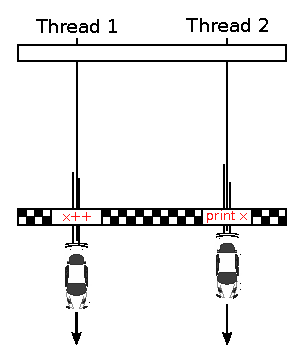
\includegraphics[scale=0.6]{pics/data-race.pdf}
					\caption*{\tiny Source: \url{https://programming.guide/go/data-races-explained.html}}
				\end{figure}
			\end{column}
		\end{columns}
	}

	\section{Background}
		\begin{frame}[fragile]
			\frametitle{Background}
			\begin{columns}
				\begin{column}{0.6\textwidth}
				\begin{lstlisting}[caption={program exhibiting a data race},language=C++]
int x;
pthread_mutex_t y;

void *Thread1(void *x) {
	x++;
	pthread_mutex_lock(&y);
	pthread_mutex_unlock(&y);
	return NULL;
}

void *Thread2(void *x) {
	pthread_mutex_lock(&y);
	x--;
	pthread_mutex_unlock(&y);
	return NULL;
}
				\end{lstlisting}
				\end{column}
				\pause
				\begin{column}{0.4\textwidth}
					\begin{table}
						\begin{center}
							\begin{tabular}{ c c c}
								& 1\# & 2\# \\
								\hline
								1. & w(x) & \\
								2. & acq(y) & \\
								3. & rel(y) & \\
								4. & & acq(y) \\
								5. & & w(x) \\
								6. & & rel(y) \\
							\end{tabular}
						\caption{obtained trace}
						\label{trace1}
						\end{center}
					\end{table}
				\end{column}
			\end{columns}
			
		\end{frame}
	
	\frame{
		\begin{columns}
			\begin{column}{0.6\textwidth}
				\Large\hspace{5em}Data race! \hspace{2em}$\Leftarrow$
			\end{column}
			\begin{column}{0.4\textwidth}
				\begin{table}
					\begin{center}
						\begin{tabular}{ c c c}
							& 1\# & 2\# \\
							\hline
							4. & & acq(y) \\
							5. & & w(x) \\
							1. & w(x) & \\
							6. &  & rel(y) \\
							2. & acq(y) & \\
							3. & rel(y) & \\
						\end{tabular}
						\caption{Trace \ref{trace1} reordered}
						\label{trace2}
					\end{center}
				\end{table}
			\end{column}
		\end{columns}
		
	}
		
	
	\frame{
		\frametitle{Background}
			\begin{itemize}
				\item dynamic data race prediction
				\item vector clocks
				\item epochs
				\item Lamport's HB relation
			\end{itemize}
	}

	
	\section{FastTrack and TSan V2}
	\frame{
		\frametitle{FastTrack and TSan V2}
		\begin{columns}
			\begin{column}{0.5\textwidth}
				\hspace{2em}FastTrack
				\begin{itemize}
					\item epoch-based
					\item semi-adaptive
				\end{itemize}
			\end{column}
			\begin{column}{0.5\textwidth}
				\centering
				ThreadSanitizer (TSan) V2
				\begin{itemize}
					\item modified version of FastTrack
					\item shadow memory
				\end{itemize}
			\end{column}
		\end{columns}
		
	}
	
	\subsection{Limitations}
	\frame{
		\frametitle{Limitations}
	}

	
	\section{Conclusion}
	\frame{
		\frametitle{Conclusion}
	}
	
\end{document}
